
\documentclass[12pt]{article}
%\renewcommand\normalsize{\fontsize{10pt}{12pt}\selectfont}
\usepackage{graphicx} % Required for inserting images
\usepackage[left=2cm,right=2cm,top=2cm,bottom=1.5cm]{geometry}

\title{HW 2}
%\author{Dennis Wilkinson}
%\date{March 31 2025; due Monday April 7}

\begin{document}

\setlength{\parindent}{0pt}
\setlength{\parskip}{3mm}

Quiz 1 solutions and explanation.

1a. The book changes from a velocity of 1.2 m/s east to 0 m/s in 2 seconds, so the acceleration is $\frac{1.2}{2} = 0.6$ m/s$^2$. The direction is against the motion, so west. I also accepted -0.6 m/s$^2$ east, though strictly speaking, magnitude should always be positive.

Key ideas: (a) the definition of acceleration, numerically speaking - $a$ is the amount $v$ changes in one second (recall m/s$^2$ means m/s, per second); and (b) accelerations need to be directed against the direction of motion to slow objects down. 

1b. You needed to calculate the time of the push (it's 1.5 seconds, since $a$ was 0.8 so it took a second and a half for the $v$ to get to 1.2) - this was similar to part a - and then draw in the graph. The lines should be straight since acceleration is constant. I asked for a specific scale on the graph, so you needed to use that for full credit.

\begin{figure}[h]
    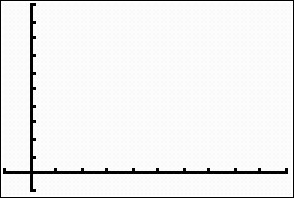
\includegraphics[width=0.4\linewidth]{GraphP1.jpg}
\end{figure}

Key ideas: making a $v$ vs $t$ graph; slope of $v$ is $a$. 

1c. Distance traveled is area under the $v$ curve; this is greater for slide than the push, so more distance was covered during the slide. Some people used a formula, which is also fine. And others used a valid conceptual argument (it spent more time slowing down, and the change in speed was the same, so it must have covered more distance) which is also fine here.

Key idea: area under the $v$ curve is distance traveled.

1d. The question is a bit vague. The book changes its acceleration from 0.8 east to 0.6 west almost instantly when the hand lets go (the repelling hard-book contact force disappears rapidly when the book and hand molecules are no longer extremely close); Since jerk is $\frac{\Delta a}{\Delta t}$, the tiny denominator makes the fraction huge. The car has a larger acceleration, but it is changing more slowly (maybe from 3-4 m/s$^2$ to 5-6 m/s$^2$ in a matter of a few seconds?) so the jerk is much less. Thus, I would argue for the book; but if you argued for the car coherently, credit was possible. However, an argument resting solely on the size of the acceleration (or the force) but not on how rapidly it changed doesn't work.

As far as the limit on jerk, this was just for fun and to get you to think. Classically, a change in $a$ is when $F$ changes; I think such a process would always take a finite amount of time, as the molecules or particles involved need to move for $F$ to change.

Key idea: rate of change of a quantity is different from the size of a quantity - like comparing the acceleration of a constant speed sports car to a turtle taking its first step.

2a. $v=0$ but $a=-9.8$ m/s$^2$, or 9.8 m/s$^2$ downward, or $g$ downward. 

Key ideas: $a$ can be nonzero even if $v$ is briefly zero; and, the acceleration of gravity is $g$ for all objects when they first start falling on Earth, before air resistance kicks in.

2b. The ball is going faster at the bottom, so it covers more ground during that half (timewise) of its path; it is thus closer than halfway to the top in altitude at time $T/2$.

Key idea: more ground is covered when speed is faster, in problems with a changing speed.

2c. No change from (a). Air resistance only exists when an object is moving. 

Key idea: air resistance doesn't exist (more accurately, there is no net force on the object) for non-moving objects. Related: air resistance force increases with increasing $v$ of the object relative to the air.

3*. After I received your answers, I realized that the technique required to solve the equation may not be taught in most HS calculus or AP physics classes - I guess you'll see it in differential equations. So if you don't understand that part, don't worry. However, writing the Newton's equation should be doable.

Here, the Newton's equation becomes $m\frac{dv}{dt}=-mkv-mg$. This can be rewritten $\frac{dv}{g+kv}=-dt$; integrating on the left from $v_0$ to 0, and on the right from 0 to $T$, gives $T=\frac{1}{k}ln(1+kv_0/g)$ after a bit of algebra. For small $k$, or strictly speaking, small $kv_0/g$, we use a Taylor series, $ln(1+kv_0/g) = kv_0/g + O((kv_0/g)^2)$ where the error is of order $(kv_0/g)^2$ or higher, to find $T \approx v_0/g$. The equality is exact in the non-air resistance case. $k$ has units of 1/time.

\end{document}